\chapter{Responsible Data Science: Ethics, Privacy, and Fairness}
\label{chap:responsible}
\chapterguide
  {You should be able to audit data quality, train and validate models, and report subgroup performance.}
  {identify ethical risks across the data lifecycle, distinguish representation and measurement problems, reason about privacy and proxy variables, compare fairness-related error rates, and document appropriate human oversight.}

\section{Technical correctness is not the same as responsible use}
A model can be reproducible, statistically accurate, and still be inappropriate for its intended context. Responsible data science asks whether the data were collected legitimately, whether relevant populations are represented, whether errors fall unevenly, whether the system creates avoidable privacy risk, and whether people can understand or challenge consequential uses.

These questions should be asked throughout the lifecycle rather than added as a final checklist after modelling.

\begin{utpfig}[Responsibility spans the whole lifecycle]{Risks enter during collection and can be amplified by later modelling, deployment, and feedback.}{fig:responsible-lifecycle}
\begin{tikzpicture}[x=\linewidth,y=1cm,
  stage/.style={draw=UTPBlue!70,fill=UTPPaleBlue,rounded corners=1.5mm,
    line width=0.6pt,text width=0.155\linewidth,minimum height=1.55cm,
    inner xsep=1.8mm,inner ysep=2mm,align=center,
    font=\scriptsize\color{UTPNavy}},
  flow/.style={-{Stealth[length=2mm,width=1.5mm]},
    line width=0.8pt,draw=UTPTeal},
  feedback/.style={flow,draw=UTPMuted,rounded corners=2mm},
  risk/.style={font=\scriptsize\color{UTPRed!85!black},align=center,
    text width=0.155\linewidth,anchor=north,inner sep=0pt}]
\node[stage] (q) at (0,0) {\textbf{Purpose}\\[4pt]
  Define the question\\and intended use};
\node[stage] (d) at (0.205,0) {\textbf{Collect}\\[4pt]
  Gather records\\and assign labels};
\node[stage] (m) at (0.410,0) {\textbf{Model}\\[4pt]
  Fit models\\and validate};
\node[stage] (a) at (0.615,0) {\textbf{Deploy}\\[4pt]
  Act on\\results};
\node[stage,draw=UTPTeal!80,fill=UTPPaleTeal] (mon) at (0.820,0)
  {\textbf{Monitor}\\[4pt]
   Review outcomes\\over time};
\draw[flow] (q.east) -- (d.west);
\draw[flow] (d.east) -- (m.west);
\draw[flow] (m.east) -- (a.west);
\draw[flow] (a.east) -- (mon.west);
\draw[feedback] (mon.north) -- (0.820,1.35) --
  node[midway,above=3pt,font=\scriptsize\color{UTPMuted}]
    {Feedback changes future data}
  (0.205,1.35) -- (d.north);
\node[risk] at (0,-1.05) {Purpose and\\necessity};
\node[risk] at (0.205,-1.05) {Consent, coverage,\\measurement};
\node[risk] at (0.410,-1.05) {Leakage, bias,\\uncertainty};
\node[risk] at (0.615,-1.05) {Error costs,\\oversight};
\node[risk] at (0.820,-1.05) {Drift and\\review};
\end{tikzpicture}
\end{utpfig}

\section{Begin with purpose and necessity}
Before collecting or modelling data, state the purpose precisely enough to test whether each data element is actually needed. This is the principle of \term{data minimisation}: collect and retain what is relevant for a defined purpose rather than accumulating fields because they might be useful someday.

A purpose statement should identify the decision or service being supported, the affected population, the expected benefit, important failure modes, and who has authority to act on the result.

\begin{workedexample}
A team building a model to estimate equipment failure risk may need sensor history, operating conditions, and maintenance records. It may not need employee names. Removing irrelevant identifiers reduces privacy exposure without weakening the analytical objective.
\end{workedexample}

\section{Representation is a property of the dataset, not the algorithm}
If some groups, environments, or operating conditions are poorly represented, model performance for them may be uncertain or systematically worse. Representation should therefore be examined before fitting.

\begin{utpfig}[Representation gaps appear before modelling]{Compare the analytical dataset with the population or environment to which conclusions will be applied. Large composition differences deserve explicit investigation.}{fig:ethics-representation}
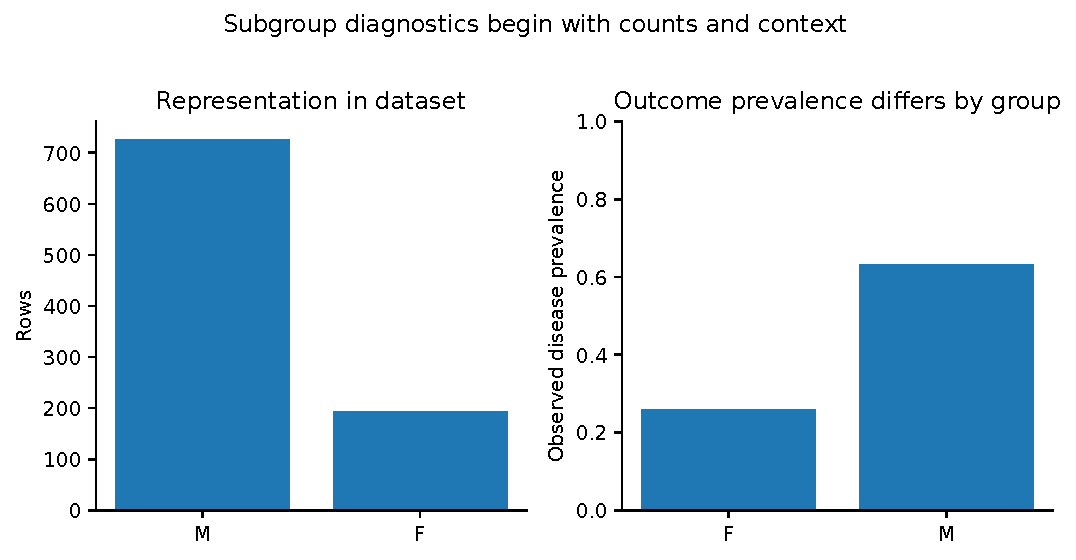
\includegraphics[width=0.80\linewidth]{figures_generated/ethics_representation.pdf}
\end{utpfig}

Small groups present a second challenge: a metric calculated from very few cases can vary greatly. Report denominators and uncertainty instead of treating every subgroup estimate as equally precise.

\section{Measurement and labels can encode human processes}
Targets and features are rarely neutral abstractions. A label may reflect a diagnostic practice, an administrative rule, a historical decision, or the behaviour of an earlier system. When labels are noisy or systematically different across groups, a model can learn those processes rather than the construct the analyst intended.

Ask:
\begin{itemize}
  \item Who or what created the label?
  \item How much disagreement exists between annotators or instruments?
  \item Could the measurement process differ by context or subgroup?
  \item Does the label measure the desired construct directly or only a proxy?
\end{itemize}

\section{Sensitive information can reappear through proxies}
Removing an explicitly sensitive field does not guarantee that the remaining features are independent of it. Location, purchasing patterns, language, school, or correlated behavioural variables can act as proxies.

\begin{utpfig}[Proxy features can retain sensitive structure]{The synthetic example uses colour only to reveal hidden group structure. A model sees the numeric proxy, not the analyst's intention when the explicit group field was removed.}{fig:ethics-proxy}
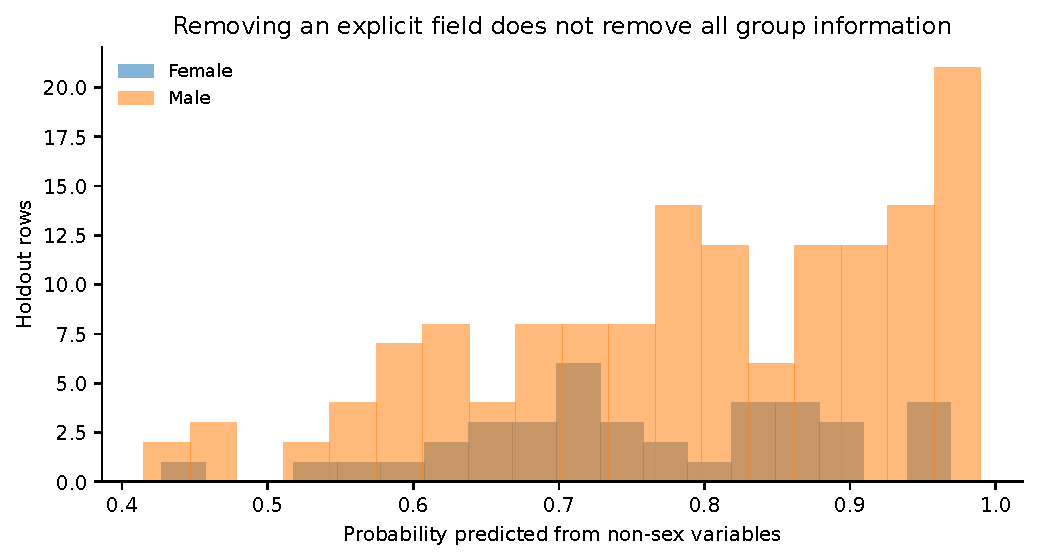
\includegraphics[width=0.76\linewidth]{figures_generated/ethics_proxy.pdf}
\end{utpfig}

\begin{pitfall}
``We removed the sensitive column'' is not a fairness analysis. The relevant question is whether model behaviour and resulting decisions differ in ways that matter across affected groups and contexts.
\end{pitfall}

\section{Privacy risk is broader than direct identifiers}
Direct identifiers such as names and account numbers are obvious risks, but combinations of quasi-identifiers can also make records distinctive. Fine-grained location, precise timestamps, rare occupations, or unusual event combinations may enable re-identification when linked with other information.

\begin{utpfig}[Re-identification can occur through linkage]{A released table without names may still contain a combination of attributes that links to an external table containing identities.}{fig:reidentification-linkage}
\begin{tikzpicture}[x=\linewidth,y=1cm,
  datacard/.style={draw=UTPBlue!70,fill=UTPPaleBlue,rounded corners=1.5mm,
    line width=0.6pt,text width=0.26\linewidth,minimum height=2.55cm,
    inner xsep=2.5mm,inner ysep=2mm,align=left,
    font=\scriptsize\color{UTPNavy}},
  flow/.style={-{Stealth[length=2mm,width=1.5mm]},
    line width=0.8pt,draw=UTPTeal}]
\node[datacard] (rel) at (0,0) {\textbf{Released data}\\[5pt]
  Birth year\\
  Postcode\\
  Event date\\
  Measurement};
\node[datacard,draw=UTPTeal!80,fill=UTPPaleTeal] (ext) at (0.335,0)
  {\textbf{External data}\\[5pt]
   \textbf{Name}\\
   Birth year\\
   Postcode\\
   Event date};
\node[datacard,draw=UTPRed!80,fill=UTPPaleRed,align=center] (id) at (0.670,0)
  {\textbf{Linked identity}\\[5pt]
   A matching record may\\
   connect a name to\\
   a released measurement};
\draw[flow] (rel.east) -- (ext.west);
\draw[flow,draw=UTPRed!80] (ext.east) -- (id.west);
\node[font=\scriptsize\color{UTPMuted},align=center,
  text width=0.85\linewidth] at (0.335,-1.75)
  {Shared linkage fields: birth year, postcode, and event date.};
\end{tikzpicture}
\end{utpfig}

Useful safeguards include minimising retained fields, reducing unnecessary precision, restricting access, separating identifiers from analytical data, defining retention periods, and reviewing whether outputs themselves reveal individual information.

\section{Pseudonymisation and anonymisation are different claims}
\term{Pseudonymisation} replaces direct identifiers with alternative identifiers but allows records to be linked under controlled conditions. \term{Anonymisation} is a much stronger claim that individuals cannot reasonably be identified from the released data. In practice, high-dimensional data make strong anonymisation difficult.

For teaching projects, the safest habit is to use public or appropriately de-identified datasets and avoid reproducing sensitive row-level examples in reports.

\section{Fairness is not a single metric}
Different fairness concepts formalise different goals. They can conflict, especially when outcome prevalence differs across groups. Therefore fairness analysis begins with the decision context and error costs, not with selecting a fashionable metric.

For a binary classifier, common quantities include:
\begin{itemize}
  \item selection or positive-prediction rate;
  \item sensitivity / true-positive rate;
  \item false-positive rate;
  \item specificity;
  \item precision / positive predictive value;
  \item calibration within groups.
\end{itemize}

\begin{utpfig}[Subgroup error rates can tell a different story from overall accuracy]{The synthetic example shows sensitivity and specificity by group. Differences may come from data quality, prevalence, sample size, threshold choice, or model fit and should be investigated rather than mechanically ``corrected''.}{fig:ethics-group-errors}
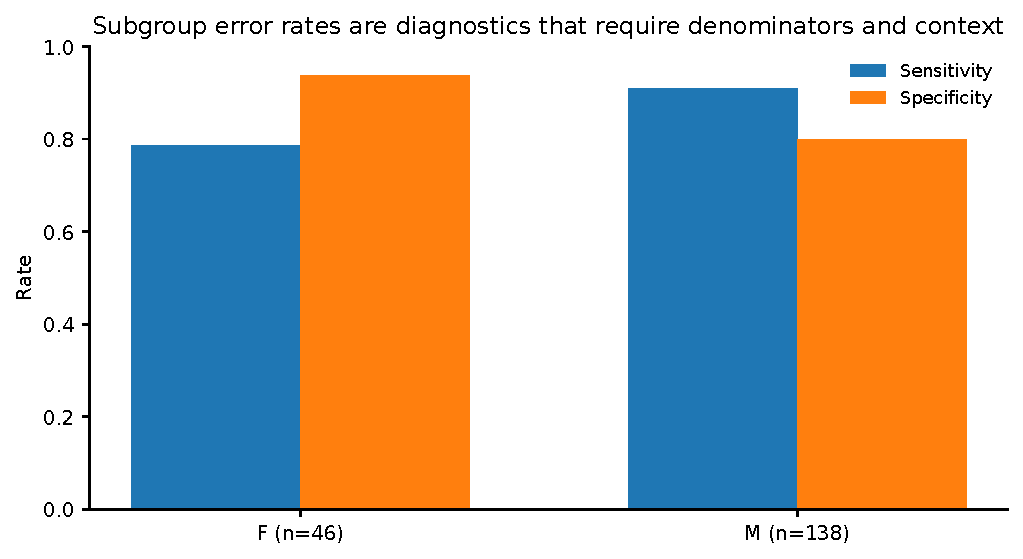
\includegraphics[width=0.82\linewidth]{figures_generated/ethics_group_error_rates.pdf}
\end{utpfig}

\section{Thresholds distribute errors}
For a probability model, changing the decision threshold changes who receives a positive classification and therefore changes false positives and false negatives. If error costs differ across people or contexts, threshold selection becomes a policy and governance decision as well as a statistical one.

\noindent\begin{minipage}{\linewidth}
\begin{utpfig}[Thresholds are decision rules, not properties of the model]{A score model produces probabilities or scores. A separate threshold converts them into actions. That separation should remain explicit in both analysis and documentation.}{fig:responsible-threshold}
\begin{tikzpicture}[x=\linewidth,y=1cm,
  stage/.style={draw=UTPBlue!70,fill=UTPPaleBlue,rounded corners=1.5mm,
    line width=0.6pt,text width=0.19\linewidth,minimum height=1.55cm,
    inner xsep=2.5mm,inner ysep=2mm,align=center,
    font=\scriptsize\color{UTPNavy}},
  flow/.style={-{Stealth[length=2mm,width=1.5mm]},
    line width=0.8pt,draw=UTPTeal}]
\node[stage] (x) at (0,0) {\textbf{Features}\\[4pt]
  Measured inputs\\for each case};
\node[stage] (m) at (0.25,0) {\textbf{Model score}\\[4pt]
  Illustrative output:\\
  score = 0.67};
\node[stage,draw=UTPOrange!80,fill=UTPPaleOrange] (t) at (0.50,0)
  {\textbf{Decision threshold}\\[4pt]
   Compare the score\\with 0.50 or 0.80};
\node[stage,draw=UTPTeal!80,fill=UTPPaleTeal] (a) at (0.75,0)
  {\textbf{Action}\\[4pt]
   Apply the chosen\\decision rule};
\draw[flow] (x.east) -- (m.west);
\draw[flow] (m.east) -- (t.west);
\draw[flow] (t.east) -- (a.west);
\node[font=\scriptsize\color{UTPRed!85!black},align=center,
  text width=0.24\linewidth,anchor=north,inner sep=0pt] at (0.50,-1.05)
  {Chosen from costs,\\capacity, and policy};
\end{tikzpicture}
\end{utpfig}
\end{minipage}\par

\section{Feedback loops can change the future training data}
Once a model influences decisions, those decisions can affect which outcomes become observable. For example, if only high-scoring cases receive an intervention, future labels may partly reflect the model's own earlier decisions. Retraining on those labels without understanding the feedback loop can reinforce existing patterns.

\begin{utpfig}[A deployment feedback loop]{Predictions influence actions, actions influence observed outcomes, and those outcomes become future training data. Monitoring must therefore examine the system, not only the model.}{fig:feedback-loop}
\begin{tikzpicture}[x=\linewidth,y=1cm,
  stage/.style={draw=UTPBlue!70,fill=UTPPaleBlue,rounded corners=1.5mm,
    line width=0.6pt,text width=0.19\linewidth,minimum height=1.55cm,
    inner xsep=2.5mm,inner ysep=2mm,align=center,
    font=\scriptsize\color{UTPNavy}},
  flow/.style={-{Stealth[length=2mm,width=1.5mm]},
    line width=0.8pt,draw=UTPTeal},
  feedback/.style={flow,draw=UTPOrange!85!black,rounded corners=2mm}]
\node[stage] (data) at (0,0) {\textbf{Historical data}\\[4pt]
  Recorded cases\\and outcomes};
\node[stage] (model) at (0.25,0) {\textbf{Model}\\[4pt]
  Learn patterns\\and predict};
\node[stage] (act) at (0.50,0) {\textbf{Decision}\\[4pt]
  Predictions guide\\actions};
\node[stage,draw=UTPTeal!80,fill=UTPPaleTeal] (out) at (0.75,0)
  {\textbf{Observed outcomes}\\[4pt]
   Actions shape what\\is observed};
\draw[flow] (data.east) -- (model.west);
\draw[flow] (model.east) -- (act.west);
\draw[flow] (act.east) -- (out.west);
\draw[feedback] (out.south) -- (0.75,-1.35) --
  node[midway,below=3pt,font=\scriptsize\color{UTPOrange!85!black}]
    {Observed outcomes become future training data}
  (0,-1.35) -- (data.south);
\end{tikzpicture}
\end{utpfig}

\section{Human oversight should be designed, not assumed}
Saying ``a human makes the final decision'' is insufficient if the human lacks time, information, authority, or a clear process for challenging the model. Effective oversight specifies what the model recommends, what evidence is shown, when review is mandatory, how disagreement is recorded, and how users can escalate unusual cases.

Automation can also create \term{automation bias}: people may over-trust a recommendation because it appears quantitative. Interfaces should therefore expose uncertainty and relevant limitations rather than only a confident label.

\section{Documentation makes limitations durable}
A responsible project records facts that future users would otherwise have to rediscover. Useful documents include a dataset sheet and a model card or model report.

\begin{dstable}
\begin{tabularx}{\linewidth}{@{}p{3.0cm}X@{}}
\toprule
\rowcolor{DSPaleBlue!92}
Document & Minimum useful content \\
\midrule
Dataset sheet & source, intended population, collection process, time coverage, exclusions, missingness, known limitations \\
Model report & target, features, training data version, validation design, metrics, subgroup checks, threshold, known failure modes \\
Decision record & intended use, prohibited or unsupported uses, reviewer, monitoring plan, retraining trigger \\
\bottomrule
\end{tabularx}
\end{dstable}

\section{A compact responsible-analysis review}
Before presenting a model or statistical result, ask:
\begin{enumerate}
  \item Is the intended use explicitly stated?
  \item Does the dataset reasonably cover the target population and operating conditions?
  \item Could labels or features encode historical decisions or measurement differences?
  \item Have privacy risks been reduced to what is necessary for the purpose?
  \item Are subgroup denominators and error rates visible where appropriate?
  \item Is uncertainty communicated instead of hidden behind one point metric?
  \item Are unsupported uses and known failure modes documented?
  \item Is there a person or process responsible for review after deployment?
\end{enumerate}

\begin{quickcheck}
\begin{enumerate}
  \item Why can representation bias exist before any model is fitted?
  \item Give an example of a proxy variable and explain why removing a sensitive field may be insufficient.
  \item Why is fairness not reducible to one universal metric?
  \item What makes human oversight meaningful rather than ceremonial?
  \item What should a model report preserve for future reviewers?
\end{enumerate}
\end{quickcheck}

\section{Responsible interpretation across the course datasets}

Ethical and professional questions are not confined to explicitly sensitive datasets. They arise whenever analysis can influence people, resources, or institutional decisions.

\begin{dstable}
\footnotesize
\begin{tabularx}{\linewidth}{@{}p{3.3cm}p{4.2cm}X@{}}
\toprule
\rowcolor{DSPaleBlue!92}
Dataset & Responsible question & Why it matters \\
\midrule
Student Performance & Could the model encode prior disadvantage or school-level differences? & Predictions about students can become self-fulfilling if used to allocate opportunity. \\
Medical Costs & Are group associations being interpreted as individual risk or causal effects? & Insurance and health variables can be sensitive and strongly confounded. \\
Heart Failure / Breast Cancer & Is a teaching classifier being mistaken for a clinical tool? & Medical deployment requires external validation, calibration, governance, and domain oversight. \\
Credit-card Fraud & Who bears the cost of false positives? & Blocking legitimate transactions creates uneven customer burden even when aggregate accuracy is high. \\
Titanic & Are historical group differences being described as context-specific rather than universal human traits? & Descriptive patterns inherit the social and historical conditions that produced the data. \\
\bottomrule
\end{tabularx}
\end{dstable}

A professional report should state the intended use and the non-use cases explicitly. ``This model predicts labels in a teaching dataset'' is a much narrower claim than ``this model can make real decisions about patients, students, or customers.''

\begin{chapterrecap}
\begin{itemize}
  \item Responsible data science begins with purpose, necessity, and affected populations.
  \item Representation, measurement, and label processes shape model behaviour before algorithm choice.
  \item Privacy risk includes linkage and indirect identifiers, not only names and IDs.
  \item Fairness analysis requires context, subgroup denominators, multiple error measures, and explicit trade-offs.
  \item Deployment creates feedback and governance responsibilities that a static validation score cannot capture.
\end{itemize}
\end{chapterrecap}
